\documentclass[10pt]{beamer}

%packages
\usepackage{babel}
\usepackage[utf8]{inputenc}
\usepackage{amsmath,tabu}
\usepackage{color}
\usepackage{tikz}
\usetikzlibrary{matrix,chains,positioning,decorations.pathreplacing,arrows}
\usetikzlibrary{fit,shapes}
\usetikzlibrary{calc,shadings}
\usepackage{pgfplots}
\usepackage{colortbl}
\usepackage{eurosym}
\usepackage{mathtools}
\usepackage{listings}
\usepackage{tabularx}

%definitions
\usepackage{algorithm,algorithmic}

%theme
\usetheme{Dresden}
\usecolortheme{rose}
\useoutertheme{tree}

%environments
\newenvironment{ExampleGer}{\begin{exampleblock}{Beispiel}}{\end{exampleblock}}

\newenvironment{customlegend}[1][]{%
	\begingroup
	% inits/clears the lists (which might be populated from previous
	% axes):
	\csname pgfplots@init@cleared@structures\endcsname
	\pgfplotsset{#1}%
}{%
	% draws the legend:
	\csname pgfplots@createlegend\endcsname
	\endgroup
}%

%definitions
\def\addlegendimage{\csname pgfplots@addlegendimage\endcsname}
% definition to insert numbers
\pgfkeys{/pgfplots/number in legend/.style={%
		/pgfplots/legend image code/.code={%
			\node at (0.295,-0.0225){#1};
		},%
	},
}

%general
\title{Combining bottom up and top down approaches for Drug-Target-Interaction prediction}
\author{Tilman Hinnerichs}
\institute{BORG - KAUST}
\date{December 09, 2019}

%presentation
\expandafter\def\expandafter\insertshorttitle\expandafter{%
	\insertshorttitle\hspace{4.5cm}%
	\insertframenumber\,/\,\inserttotalframenumber
}

\definecolor{myblue}{RGB}{80,80,160}
\definecolor{mygreen}{RGB}{80,160,80}
\definecolor{myturk}{RGB}{240,60,60}

\begin{document}
	
\begin{frame}
	\titlepage
\end{frame}

\begin{frame}{Outline}
	\setbeamertemplate{section in toc}[sections numbered]
	\tableofcontents
\end{frame}

\section{Problem Description}
\begin{frame}{Problem Description}
	Prediction over bipartite graph:
	
	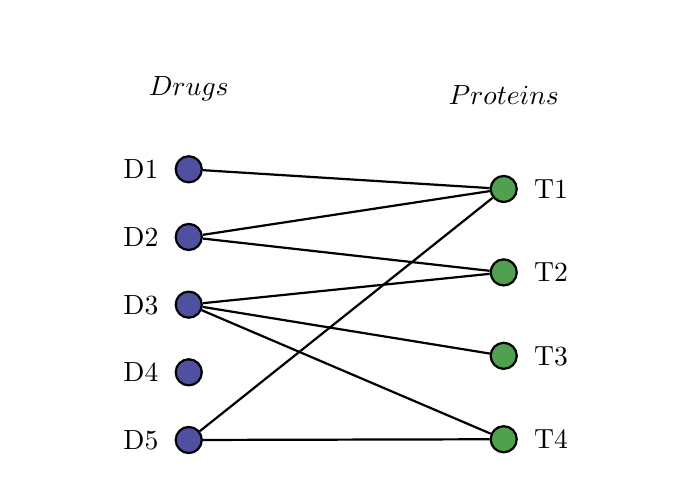
\begin{tikzpicture}[thick,
	every node/.style={draw,circle},
	fsnode/.style={fill=myblue},
	fs1node/.style={fill=myblue},
	ssnode/.style={fill=mygreen},
	%every fit/.style={ellipse,draw,inner sep=-1pt,text width=2cm},
	%->,shorten >= 3pt,shorten <= 3pt
	]
	
	% the vertices of U
	\begin{scope}[start chain=going below,node distance=5mm]
	\foreach \i in {1,2,...,3}
	\node[fsnode,on chain] (f\i) [label=left: D\i] {};
	\end{scope}
	
	% the vertices of U1
	\begin{scope}[node distance=5mm]
	\foreach \i in {4,5}
	\node[fs1node,on chain] (f\i) [label=left: D\i] {};
	\end{scope}
	
	% the vertices of V
	\begin{scope}[xshift=4cm,yshift=-0.25cm,start chain=going below,node distance=7mm]
	\foreach \i in {1,2,...,4}
	\node[ssnode,on chain] (s\i) [label=right: T\i] {};
	\end{scope}
	
	% the set U
	%\node [myblue, fit=(f1) (f3)] {};
	\node [white,fit=(f1) (f5),label=above:$Drugs$] {};
	
	% the set V
	\node [white,fit=(s1) (s4),label=above:$Proteins$] {};
	
	% the edges
	\draw (f1) -- (s1);
	\draw (s1) -- (f2);
	\draw (f2) -- (s2);
	\draw (s2) -- (f3);
	\draw (s3) -- (f3);
	\draw (f3) -- (s4);
	\draw (s4) -- (f5);
	\draw (f5) -- (s1);
	\end{tikzpicture}
	
\end{frame}


\begin{frame}{Classification of recent approaches\footnote{Chen Wang et al., Briefings in Bioinformatics, 2018}\footnote{Yu Ding et al., Briefings in Bioinformatics, 2019}}
	\begin{table}
		\begin{tabularx}{\textwidth}{|>{\setlength\hsize{.5\hsize}\setlength\linewidth{\hsize}}X|>{\setlength\hsize{1.25\hsize}\setlength\linewidth{\hsize}}X|>{\setlength\hsize{1.25\hsize}\setlength\linewidth{\hsize}}X|}
			\hline
			&Drugs&Protein\\
			\hline
			bottom-up&
			\begin{itemize}
				\item GCN over molecules
				\item drug similarity
			\end{itemize}&
			\begin{itemize}
				\item secondary structure prediction
				\item contact prediction
				\item convolution over amino acid sequences
			\end{itemize}\\
			\hline
			top-down&
			\begin{itemize}
				\item network approaches
				\item drug similarity
			\end{itemize}&
			\begin{itemize}
				\item protein similarity
			\end{itemize}\\
			\hline
		\end{tabularx}
	\end{table}	
\end{frame}

\begin{frame}{Problems of recent approaches}
	Main issues:
	\begin{itemize}
		\item Lack ability to generalize or are unable to spot small differences
		\item Usually only top-down or bottom-up
		\item Not making use of interaction networks
	\end{itemize}
	\pause
	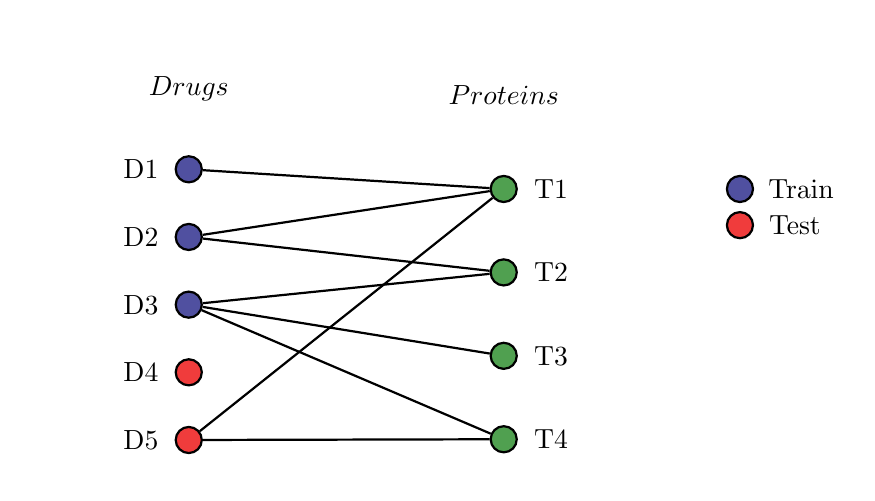
\begin{tikzpicture}[thick,
	every node/.style={draw,circle},
	fsnode/.style={fill=myblue},
	fs1node/.style={fill=myturk},
	trainlegendnode/.style={fill=myblue},
	testlegendnode/.style={fill=myturk},
	ssnode/.style={fill=mygreen},
	%every fit/.style={ellipse,draw,inner sep=-1pt,text width=2cm},
	%->,shorten >= 3pt,shorten <= 3pt
	]
	
	% the vertices of U
	\begin{scope}[start chain=going below,node distance=5mm]
	\foreach \i in {1,2,...,3}
	\node[fsnode,on chain] (f\i) [label=left: D\i] {};
	\end{scope}
	
	% the vertices of U1
	\begin{scope}[node distance=5mm]
	\foreach \i in {4,5}
	\node[fs1node,on chain] (f\i) [label=left: D\i] {};
	\end{scope}
	
	% the vertices of V
	\begin{scope}[xshift=4cm,yshift=-0.25cm,start chain=going below,node distance=7mm]
	\foreach \i in {1,2,...,4}
	\node[ssnode,on chain] (s\i) [label=right: T\i] {};
	\end{scope}
	
	% legend
	\begin{scope}[xshift=7cm,yshift=-0.25cm,start chain=going below,node distance=7mm]
	\foreach \i in {1}
	\node[trainlegendnode,on chain] (trainlegend\i) [label=right: Train] {};
	\end{scope}
	
	\begin{scope}[xshift=7cm,yshift=-0.25cm, node distance=1mm]
	\foreach \i in {1}
	\node[testlegendnode,on chain] (testlegend\i) [label=right: Test] {};
	\end{scope}
	
	% the set U
	%\node [myblue, fit=(f1) (f3)] {};
	\node [white,fit=(f1) (f5),label=above:$Drugs$] {};
	
	% the set V
	\node [white,fit=(s1) (s4),label=above:$Proteins$] {};
	
	% the edges
	\draw (f1) -- (s1);
	\draw (s1) -- (f2);
	\draw (f2) -- (s2);
	\draw (s2) -- (f3);
	\draw (s3) -- (f3);
	\draw (f3) -- (s4);
	\draw (s4) -- (f5);
	\draw (f5) -- (s1);
	\end{tikzpicture}
	
\end{frame}


\begin{frame}{Features in context}
	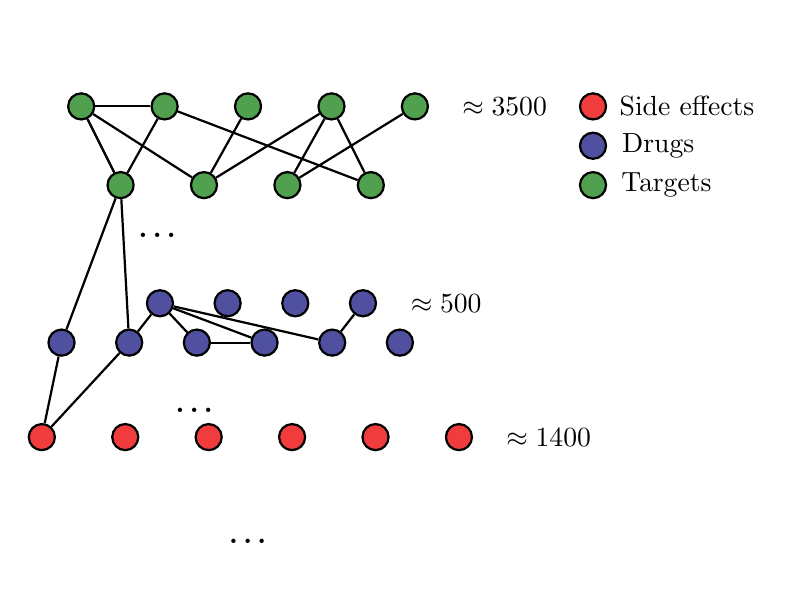
\begin{tikzpicture}[thick,
	every node/.style={draw,circle},
	fsnode/.style={fill=myblue},
	fs1node/.style={fill=myturk},
	drughierarchynode/.style={fill=myturk},
	druglegendnode/.style={fill=myblue},
	hierarchylegendnode/.style={fill=myturk},
	targetlegendnode/.style={fill=mygreen},
	ssnode/.style={fill=mygreen},
	%every fit/.style={ellipse,draw,inner sep=-1pt,text width=2cm},
	%->,shorten >= 3pt,shorten <= 3pt
	]
	
	% the vertices of U
	\begin{scope}[xshift=2.25cm,yshift=-3cm,start chain=going right,node distance=5mm]
	\foreach \i in {1,2,...,6}
	\node[fsnode,on chain] (f\i) {};
	\end{scope}
	
	\begin{scope}[xshift=3.5cm,yshift=-2.5cm,start chain=going right,node distance=5mm]
	\foreach \i in {7,8,...,10}
	\node[fsnode,on chain] (f\i) {};
	\end{scope}
	
	% Hierarchy nodes
	\begin{scope}[xshift=2cm,yshift=-4.2cm,start chain=going right,node distance=7mm]
	\foreach \i in {1,2,...,6}
	\node[drughierarchynode,on chain] (dh\i) {};
	\end{scope}
	
	
	% the vertices of V
	\begin{scope}[xshift=2.5cm,yshift=0cm,start chain=going right,node distance=7mm]
	\foreach \i in {1,2,...,5}
	\node[ssnode,on chain] (s\i) {};
	\end{scope}
	\begin{scope}[xshift=3cm,yshift=-1cm,start chain=going right,node distance=7mm]
	\foreach \i in {6,7,...,9}
	\node[ssnode,on chain] (s\i) {};
	\end{scope}
	
	% legend
	\begin{scope}[xshift=9cm,yshift=0cm, node distance=1mm]
	\foreach \i in {1}
	\node[hierarchylegendnode] (hlegend\i) [label=right: Side effects] {};
	\end{scope}
	\begin{scope}[xshift=9cm,yshift=-0.5cm, node distance=1mm]
	\foreach \i in {1}
	\node[druglegendnode] (dlegend\i) [label=right: Drugs] {};
	\end{scope}
	\begin{scope}[xshift=9cm,yshift=-1cm, node distance=1mm]
	\foreach \i in {1}
	\node[targetlegendnode] (tlegend\i) [label=right: Targets] {};
	\end{scope}
	
	
	\node [white, fit=(dh3) (dh4),label=below:$\textbf{\dots}$] {};
	\node [white, fit=(f3),label=below:$\textbf{\dots}$] {};
	\node [white,fit=(f7), label=above:$\textbf{\dots}$] {};
	
	\node [white,fit=(s5), label=right:$\approx3500$] {};
	\node [white,fit=(f10), label=right:$\approx500$] {};
	\node [white,fit=(dh6), label=right:$\approx1400$] {};
	
	
	% the set U
	%\node [myblue, fit=(f1) (f3)] {};
	
	% DTI edges
	\draw (f1) -- (s6);
	\draw (f2) -- (s6);
	
	% PPI edges
	\draw (s1) -- (s6);
	\draw (s1) -- (s2);
	\draw (s1) -- (s6);
	\draw (s1) -- (s7);
	\draw (s2) -- (s6);
	\draw (s4) -- (s9);
	\draw (s3) -- (s7);
	\draw (s4) -- (s8);
	\draw (s4) -- (s7);
	\draw (s2) -- (s9);
	\draw (s5) -- (s8);
	
	% DDI edges
	\draw (f3) -- (f7);
	\draw (f4) -- (f7);
	\draw (f5) -- (f7);
	\draw (f3) -- (f4);
	\draw (f5) -- (f10);
	\draw (f2) -- (f7);
	
	% Side effect edges
	\draw (f1) -- (dh1);
	\draw (f2) -- (dh1);
	
	
	\end{tikzpicture}
\end{frame}

\begin{frame}{Available data structures}
	$\rightarrow$ Combine Bottom up and top down features for drugs and features
	Data structures used:
	\begin{itemize}
		\item PPIs, DTIs
		\item Motifs along proteins
		\begin{itemize}
			\item find motif along protein sequences with HMMs for each drug
		\end{itemize}
		\item DeepGO embeddings
		\item DDIs, SIDER, MedDRA
		\item DL2vec
		\item Seq2seq for drugs	
	\end{itemize}
\end{frame}

\begin{frame}{Drugs}
	\begin{itemize}
		\item matrix[drug\_index]
		\item semantic similarities over MedDRA
		\item Seq2seq from Smiles
		\item DL2vec over SIDER-MedDRA-HPO
	\end{itemize}
\end{frame}

\begin{frame}{Proteins}
	\begin{itemize}
		\item DeepGO
		\item Motifs from HMM
		\item DL2vec Embeddings from Azza and Jun
		\item node degree percentile (Gray encoding)
		\item GNNs (node features):
		\begin{itemize}
			\item Motifs from HMM
			\item DDI induced targets
			\item semantic similarity weighted targets
			\item DL2vec embeddings from Azza and Jun
			\item DL2vec over HPO/MP/MedDRA
			\item DL2vec over PhenomeNET (GO,MP/HPO, SIDER)
		\end{itemize}
	\end{itemize}
\end{frame}

\begin{frame}{Architectures}
	\begin{itemize}
		\item every possible layer from PyG
		\item Node features with/without GNN
		\item cat([drug\_feat, prot\_feat]) as (node-) feature
		\item siamese over drugs and proteins/their (graph-)embeddings
	\end{itemize}
	\pause 
	Not included:
	\begin{itemize}
		\item Variations of all datasets
	\end{itemize}
\end{frame}


\end{document}